
\documentclass[twocolumn, amsmath]{revtex4}

\usepackage{graphicx}
%\graphicspath{ {tex_pics/} }


\begin{document}


\title{PHYS 605 Lab \#7} 

\author{Morgan A. Daly}
\author{Evin O'Shea}
\date{\today} 


\maketitle


\section{Introduction and Theory}
\subsection{Purpose}

The goal of part A of the lab was to investigate the internal resistance of the ProtoBoard's AC voltage supply. This improved understanding of output voltage and output impedance of a circuit. 

Part B of the lab involved investigating the output impedance of an operational amplifier circuit. In this case the circuit was an inverting amplifier with a gain of -3. The design and testing of the circuit required an understanding of the limitations of the amplifier and the effect that a change in any of the resistor values might have, including adding a load.

Part C of the lab was to build another operational amplifier circuit. The circuit's behavior was investigated by measuring output voltage while varying input frequency. 

\subsection{Background / Theory}

The magnitude of the output impedance of a circuit, $R_0$ can be found by measuring the output voltage of a circuit with no load, $V_0$, and then measuring the output voltage with a load, $V_L$. 
The voltage of the source is measured when the output voltage is measured without the load. 
When the load is applied, the current can be calculated using the load resistance and the voltage across the load. This can be  used to calculate the output impedance.

\begin{equation}
R_{0} =  \frac{V_{R_{0}}}{I_{L}} = (V_{0} - V_{L})\frac{R_{L}}{V_{L}}
\end{equation}

The output impedance and voltage of a circuit can help determine other aspects of the circuits behavior. 
% ACTIVE VS PASSIVE CIRCUIT??
When a voltage is being supplied from an active circuit to a load, the output impedance can tell a lot about the limitations of the loads that can be used. 
If the output impedance of a passive circuit is much higher than the impedance of the circuit load, then sag can occur. This is usually something that should be avoided.

\begin{figure}[h]
    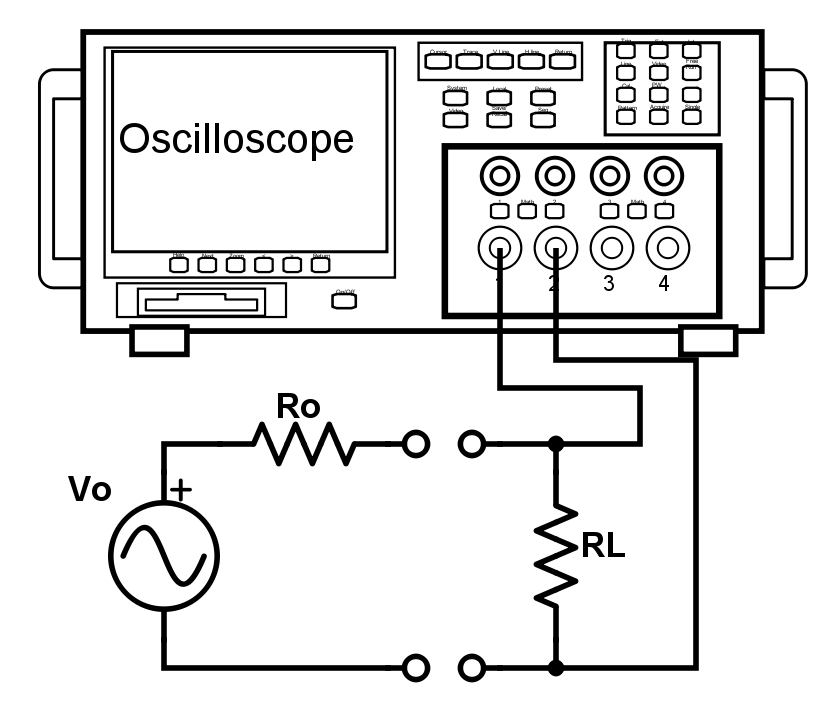
\includegraphics[scale=0.25]{output.png}  
    \caption{A circuit that can be used to take measurements in order to calculate the Norton current. If $V_0$ is measured separately, this can be used to find $R_0$.}
\end{figure}

This type of measurement can be made on other types of circuits. For the second part of the lab, the same set up can be used where $V_{o}$ and $R_{o}$ are the output voltage and output impedance of the circuit created for the second part of the lab.

Operational amplifiers are active circuit elements that can be used in a multitude of ways. An important property of the "op amp" is that its positive and negative terminals will be equal in potential. As a result, when the positive terminal is grounded, the voltage of both terminals will be zero. This implies that $\frac{V_{in}}{R_{in}} = -\frac{V_{out}}{R_{F}}$. The relationship can also be used to calculate the gain:

\begin{equation}
gain =  \frac{V_{out}}{V_{in}} = -\frac{R_{F}}{R_{in}}
\end{equation}


\begin{figure}[h]
    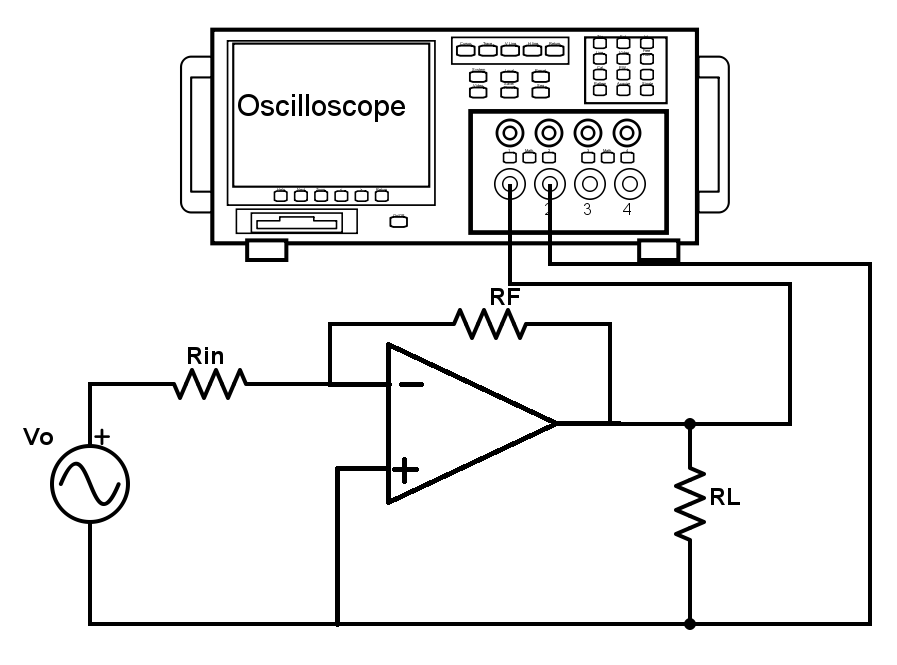
\includegraphics[scale=0.3]{inverting.png}  
    \caption{Diagram of an inverting amplifier.}
\end{figure}

It is also possible to combine a filter with an amplifier, as shown in figure (3). The circuit depicted is a high pass filter, as only high frequency voltages are able to pass through. In a DC circuit, a capacitor would not let current flow after it is charged. In an AC circuit, the change in the voltage on one side of the capacitor will cause change in voltage on the other side, allowing the AC current to continue to flow. 
Since the capacitor responds to changes in voltage, higher frequency voltages will pass through the circuit more easily than low frequency voltages. 
%???
In this circuit there is a negative feedback, so the positive and negative terminals of the op amp will have an equal voltage. Because the positive terminal is grounded, the voltage of both terminals will both be 0V. The gain of this circuit will be determined by

\begin{equation}
gain =  -\frac{Z_{F}}{Z_{in}} \,
\end{equation}

where, $Z_{in} = R_{in} + C_{in}$. The magnitude of this gain will depend on the frequency of the input voltage. The filter will allow high frequency voltages to pass and low frequencies will have a gain of less than one. The characteristic frequency of an RC circuit is given by:

\begin{equation}
\omega_{RC} =  \frac{1}{R_{in}C_{in}}
\end{equation}


\begin{figure}[h]
    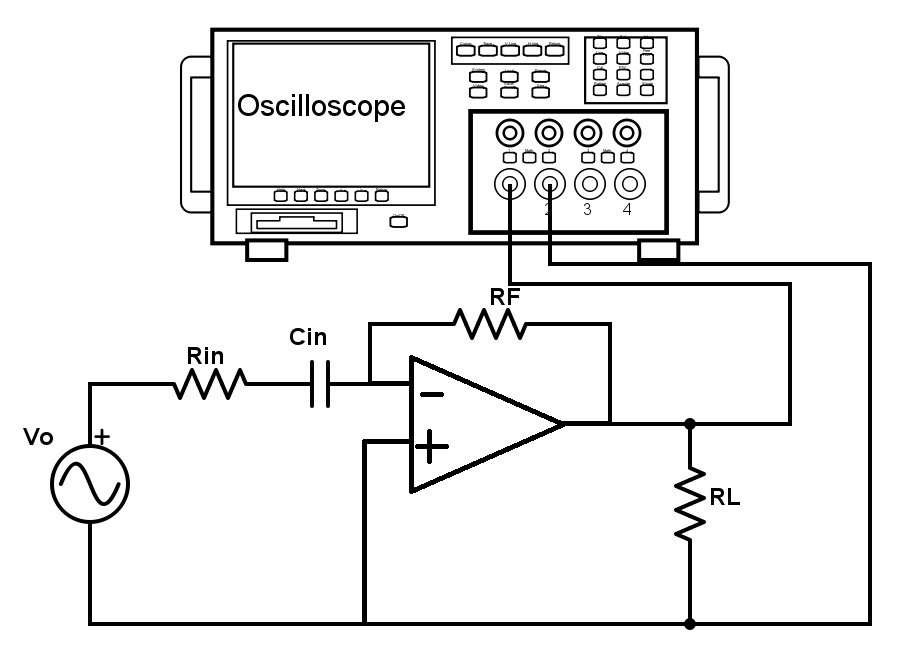
\includegraphics[scale=0.3]{highpassamp.png}  
    \caption{This circuit acts as both a high pass filter and an amplifier.}
\end{figure}


\section{Methodology}

\begin{enumerate}
    \item Connect the oscilloscope directly to the ProtoBoard's AC voltage supply and measure the output voltage.
    \item Set up the circuit shown in figure (1) record the voltage across the resistor and record the resistor value
    \item Build the op amp circuit from figure (2).
    \item Take record of the output voltage with no load attached.
    \item Add a load to the circuit with a large value as to eliminate sag.
    \item Measure the voltage across the load resistor and the value of this resistor.
    \item Change the frequency and take nots on any changes in the plot on the oscilloscope.
    \item Change the load resistor and investigate the limitations of the circuit.
    \item Build the circuit from figure (3).
    \item Take recordings of output voltage as the frequency is varied and the input voltage is kept constant.
\end{enumerate}


\section{Results and Analysis}

\subsection{Data}
The goal of part A of the lab was to make measurements to calculate the internal resistance of the AC voltage source on the ProtoBoard. 

\begin{center}
	\begin{ruledtabular}
    \begin{tabular}{ l l l }
	$V_{o}$ (V) & $V_{L}$ (V) & $R_{L}$ (k$\Omega$) \\ \colrule
	3.76 & 3.64 & 22.23  \\
	3.76 & 3.70 & 148.4  \\
	3.76 & 1.04 & 0.2184  \\
	3.76 & 3.68 & 82.1  \\
\end{tabular}
    \end{ruledtabular}
\end{center}

The goal of the second part of the lab was to build and investigate an inverting amplifier circuit. The $R_{in}$ used was 4.912k$\Omega$ and the $R_{F}$ used was 14.62k$\Omega$.

\begin{center}
	\begin{ruledtabular}
    \begin{tabular}{ l l l }
	Load & $V_{L}$ (V) & $R_{L}$ (k$\Omega$) \\ \colrule
	no load & 3.64 & 22.23  \\
	 & 3.70 & 148.4  \\
	3.76 & 1.04 & 0.2184  \\
	3.76 & 3.68 & 82.1  \\
\end{tabular}
    \end{ruledtabular}
\end{center}

The lab group also made a circuit with double the values for $R_{in}$ and $R_{F}$. For this part of the lab, $R_{in}$ = 9.811k$\Omega$, $R_{F}$ = 29.38k$\Omega$. For a measured $V_{in}$ = 1.00V yielded a $V_{out}$ = 2.947.

For part C of the lab, the group built a high pass filter and amplifier circuit using the op amp. The input voltage used for this section was 1V peak-to-peak. It used a capacitor $C_{in}$=99nF and resistor $R_{in}$=2.183$k\Omega$. The $R_F$ was 4.428$k\Omega$. The data recorded is shown below:

\begin{center}
	\begin{ruledtabular}
    \begin{tabular}{ l l }
	frequency (Hz) & $V_{out}$ (V) \\ \colrule
	102000 & 1.76 \\
	92590 & 1.84  \\
	58140 & 1.92 \\
	2119 & 1.88 \\
	1000 & 1.64 \\
	735.3 & 1.46 \\
	457.8 & 1.16 \\
	102 & 0.324 \\
	52.63 & 0.168 \\
	10.75 & 0.044 \\
\end{tabular}
    \end{ruledtabular}
\end{center}


\subsection{Calculations}

The objective of the first part of the lab was to find the internal resistance of the ProtoBoard AC voltage supply. To do this, the group measured the output directly and the output across a load. The group then used equation (1) to obtain the internal resistance of the voltage source.
$$R_{0} = (3.76 - 3.64)\frac{22.23}{3.36}=0.73$$


\begin{center}
	\begin{ruledtabular}
    \begin{tabular}{ l l l }
	$V_{L}$ (V) & $R_{L}$ (k$\Omega$) & $R_{o}$ (k$\Omega$) \\ \colrule
	3.64 & 22.23 & 0.73 \\
	3.70 & 148.4 & 2.41 \\
	1.04 & 0.2184 & 0.571 \\
	3.68 & 82.1 & 1.78 \\
\end{tabular}
    \end{ruledtabular}
\end{center}

From these calculations of $R_{0}$ the average was calculated. 
$$R_{0_{ave}} = 1.37k\Omega$$

For part B, the gain was calculated using equation (2). 
$$gain = -\frac{14620}{4912} = -2.98$$
When no load was applied, for a $V_{in}$ = 1.0V, an output of $V_{out}$ = 3.02V with an inverted signal was obtained. This is a 1.34\% error on the magnitude of the gain. When a 22.22k$\Omega$ load was added, the output voltage for a $V_{in}$ = 1.0V was $V_{out}$ = 2.97V with an inverted signal. This gives a 0.33\% error in the gain. The output resistance can be calculated for this circuit using equation (1), as in part A of the lab. In this case: $V_{o}$ = 3.02V, $V_{L}$ = 2.97V, $R_{L}$ = 22.22k$\Omega$. The result from applying equation (1) yields: 

$$R_{o} =  \frac{V_{R_{o}}}{I_{L}} = (3.02 - 2.97)\frac{22.22}{2.97} = 0.367k\Omega$$

When the resistor values were changed to $R_{in}$ = 9.811k$\Omega$ and $R_{F}$ = 29.38k$\Omega$ the expected gain of the circuit was -2.99. Since the actual gain was 2.95, the error in the gain was 1.44\%. 

For Part C of the lab, the gain of the op amp unit is 0 for very small $\omega$. The characteristic frequency was calculated using equation (4):
$$ \omega_{RC} =  \frac{1}{(2183)(99.7\times10^{-9})}=4594.64 $$

For $\omega >> \omega_{RC}$,
$$gain = \frac{-4428}{2183} \, .$$
Below is the gain calculated with equation (2) to compare:

\begin{center}
	\begin{ruledtabular}
    \begin{tabular}{ l l }
	frequency (Hz) & gain (dB) \\ \colrule
	102000 & 4.91 \\
	92590 & 5.30  \\
	58140 & 5.67 \\
	2119 & 5.48 \\
	1000 & 4.30 \\
	735.3 & 3.29 \\
	457.8 & 1.29 \\
	102 & -9.80 \\
	52.63 & -15.5 \\
	10.75 & -27.1 \\
\end{tabular}
    \end{ruledtabular}
\end{center}



\subsection{Analysis}
For part A, the group found that $R_{0_{ave}}$ = 1.37k$\Omega$. This value is in the range of values obtained. It seems as though the ProtoBoard did not have the precision to accurately measure the voltages to a degree which would allow the calculations to be consistent. With a better measurement device, the data would likely have been more precise.

The goal of part B of the lab was to build an inverting amplifier with a gain of -3. When the group initially built the circuit, $R_{in}$ = 4.912k$\Omega$ and $R_{F}$ = 14.62k$\Omega$. This gave an expected gain of -2.98. The gain obtained was -3.02. This is a 1.34\% error on the magnitude of the gain. When a load of 22.22k$\Omega$ was added, the gain was 2.97. This is a 0.33\% error. This demonstrates that the inverting amplifier achieved the goal of a gain of -3. 

The lab group then investigated the limitations on the load values. Since the output was measured with the oscilloscope attached and no load and there were no problems, it means that the circuit could handle very large loads. When a load of 47.5$\Omega$ was added, the output voltage was capped. This meant that the load resistance was too low and this was causing sag. The circuit is limited to large loads. 

The lab group then investigated what changing the resistance values does to the circuit if the ratio between them is maintained. For this part of the lab the group doubled the resistance values to $R_{in}$ = 9.811k$\Omega$ and $R_{F}$ = 29.38k$\Omega$. The expected gain for this circuit was -2.99. The gain calculated from measurements was -2.95. This is a percent error of  1.44\%. The minimal amount of error shows that changing the resistance values does not change the gain of the circuit. It was noted that increasing the resistance this way will increase the power consumption of the circuit.

For part C of the lab the group built a high pass filter and amplifier circuit using the op amp. For this circuit, a Bode plot was constructed to illustrate the circuit behavior.

\begin{figure}[h]
    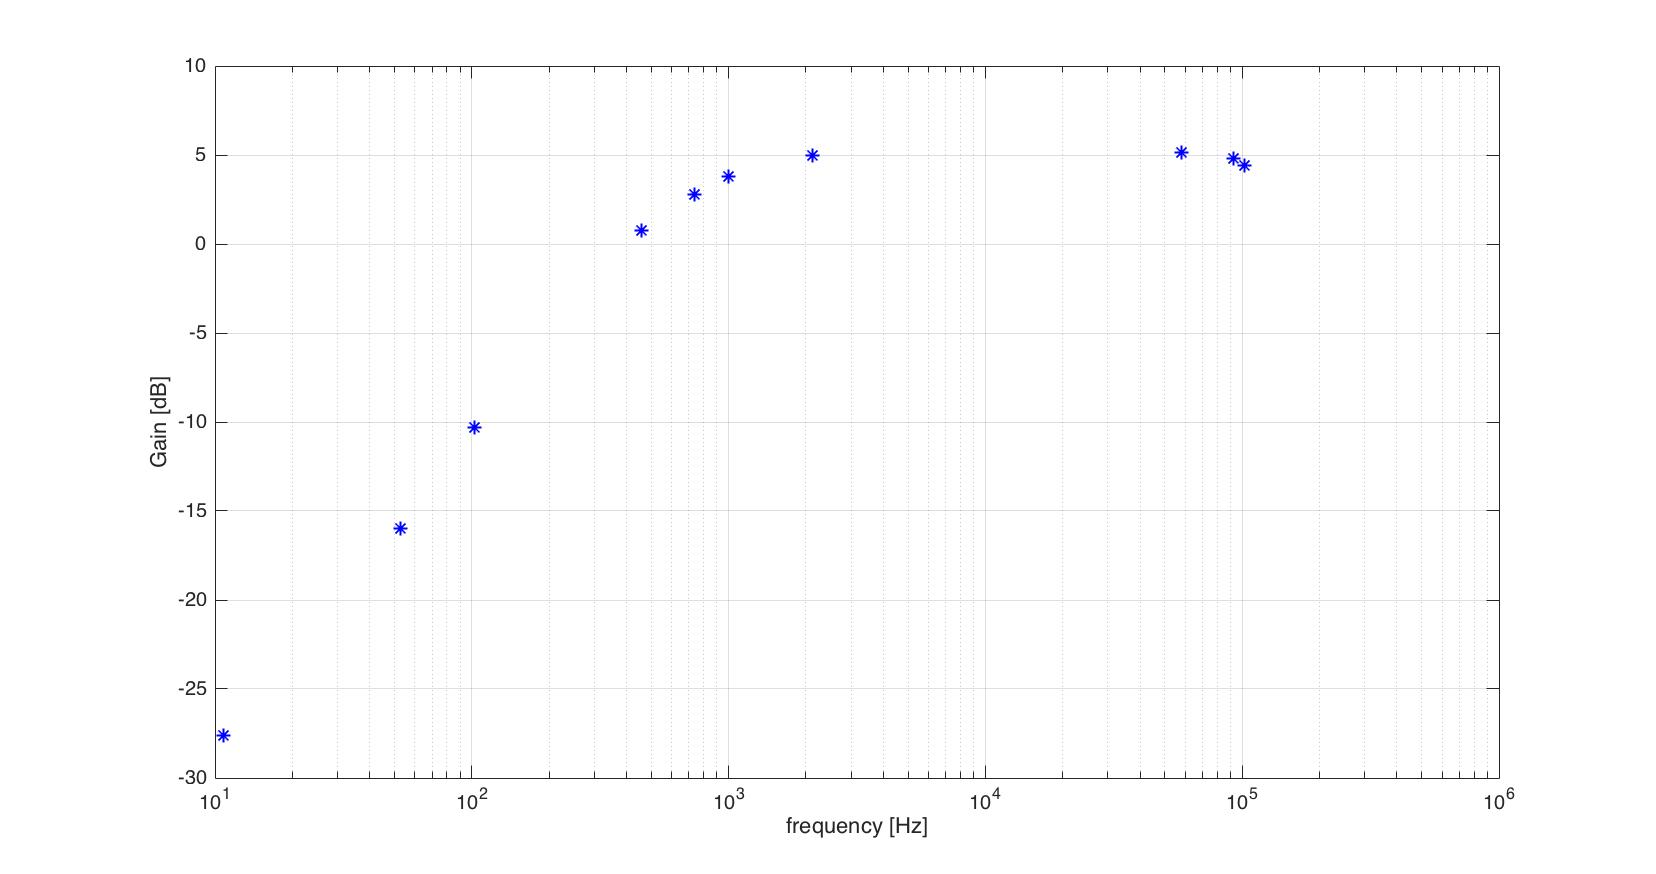
\includegraphics[scale=0.15]{bode_plot.jpg}  
    \caption{Bode plot of the high pass amplifier.}
\end{figure}

At the characteristic frequency, 4594.64, the gain is approximately -3dB, which is what was expected. The plot demonstrates that the gain in dB is negative for the frequencies below $\omega_{RC}$. This means that the low frequencies are filtered and the high frequencies are passed through the filter. This is the exact nature expected for a high pass filter. An interesting aspect is the positive gain for higher frequencies. This is the result of the amplifying element of the circuit, not only passing through higher frequencies, but amplifying their voltage.

\section{Conclusion}
Part A of the lab was successfully completed, as the internal resistance of the voltage source was calculated. None of the calculated values were very different from the average value. The lab could be improved with a better measurement device for the voltages and by taking more measurements using different load sizes.

The goal of Part B of the lab was to build and investigate the inverting amplifier. The group successfully obtained a gain of negative three with a low percent error in all cases. The group also showed that the circuit was limited to large loads as expected. The group also showed that changing the resistance values does not change the gain of the amplifier if the ratio is held constant. All of the goals of this section of the lab were completed successfully.

Part C of the lab was completed successfully, as the group built an op amp circuit that showed the desired output. The group collected data that showed the nature of the circuit to be a high pass filter, as well as an amplifier.


\end{document}

